\documentclass[10.5pt,a4paper]{article}
\usepackage[margin=2cm]{geometry}
\usepackage[T1]{fontenc}
\usepackage{lmodern,amssymb,booktabs,array,graphicx,float,caption}
\usepackage[hidelinks]{hyperref}
\usepackage{listings,xcolor}
\lstset{basicstyle=\ttfamily\scriptsize,frame=single,columns=fullflexible,keepspaces=true,
  backgroundcolor=\color{gray!8},rulecolor=\color{gray!50},aboveskip=3pt,belowskip=3pt}
\renewcommand{\arraystretch}{1.2}\setlength{\tabcolsep}{5pt}
\newcolumntype{L}[1]{>{\raggedright\arraybackslash}p{#1}}
\captionsetup{font=small,skip=3pt}
\graphicspath{{partE_screenshots/}}
\title{CRASH: Collision Risk Analysis through Semantic Hierarchies\\[4pt]\large AI-3001 Iteration 1 --- Part E: SPARQL Queries and Symbolic Reasoning}
\author{Team members: Ritaj, Hamna, Tahreem}\date{November 2026}
\begin{document}\maketitle
\section{Setup}
All queries were run in the GraphDB repository \texttt{CRASH} (OWL2-RL ruleset, schema and data from Part D, R7 HighRiskArea already inserted, 30 LSOAs) with ``Include inferred'' switched on. Every query uses the prefixes below. Ten queries cover basic graph patterns, FILTER, OPTIONAL, UNION, aggregation, multi-hop traversal, property paths and inference. Results were first computed in a separate rdflib + owlrl run and then compared with GraphDB.
\begin{lstlisting}
PREFIX : <https://crash.example.org/ontology#>
PREFIX res: <https://crash.example.org/resource/>
\end{lstlisting}
\begin{table}[H]\centering\small
\begin{tabular}{L{1.1cm} L{6.6cm} L{4.2cm} c}
\toprule
\textbf{Query} & \textbf{Purpose} & \textbf{Rows (GraphDB)} & \textbf{Match}\\
\midrule
Q1 & Fatal, speed 60+ & 19 & \checkmark \\
Q2 & VRU vehicle types (CQ1) & 19 & \checkmark \\
Q3 & Top 5 LAs, A road wet/icy (CQ2) & 5 & \checkmark \\
Q4 & HighRiskArea + force (CQ3) & 30 & \checkmark \\
Q5 & Ped/cyclist KSI casualties & 2 & \checkmark \\
Q6 & High-risk LSOAs per LA & 11 & \checkmark \\
Q7 & Gwent KSI and VRU (CQ6) & 1 & \checkmark \\
Q8 & KSI+VRU per risk area (CQ13) & 26 & \checkmark \\
Q9 & One collision record (CQ12) & 1 & \checkmark \\
Q10 & Motorcyclist KSI, 50+ (CQ10) & 62 & \checkmark \\
\bottomrule\end{tabular}\end{table}
All ten queries returned exactly the row counts and top rows we expected, so there are no mismatches.
\section{SPARQL queries}
\subsection*{Q1. Fatal collisions on roads with a speed limit of 60 or more.}
\textbf{Features:} basic graph pattern, FILTER.
\begin{lstlisting}
SELECT ?c ?date ?roadClass ?speed WHERE {
  ?c a :FatalCollision ; :collisionDate ?date ; :roadClass ?roadClass ; :speedLimit ?speed .
  FILTER(?speed >= 60)
} ORDER BY ?date
\end{lstlisting}
\begin{figure}[H]\centering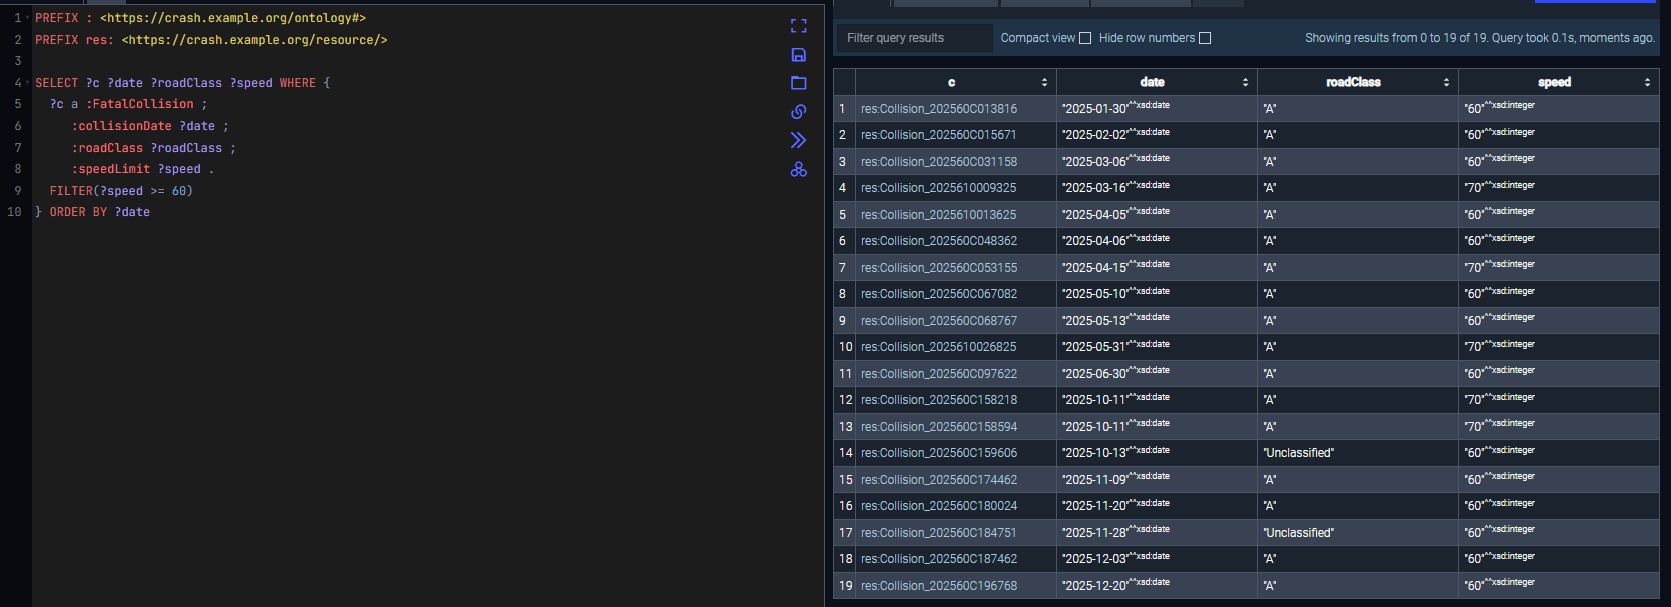
\includegraphics[width=\linewidth]{q1.png}\caption{Q1 in GraphDB.}\end{figure}
\textbf{Observed:} 19 rows, same as expected. First row Collision\_202560C013816 (2025-01-30, A, 60). Two rows have road class Unclassified.

\subsection*{Q2. Vehicle types in collisions that involved a vulnerable road user (CQ1).}
\textbf{Features:} multi-hop, aggregation, inference (VRUCollision).
\begin{lstlisting}
SELECT ?vehicleType (COUNT(DISTINCT ?c) AS ?collisions) WHERE {
  ?c a :VRUCollision ; :hasVehicle ?v .
  ?v :vehicleType ?vehicleType .
} GROUP BY ?vehicleType ORDER BY DESC(?collisions)
\end{lstlisting}
\begin{figure}[H]\centering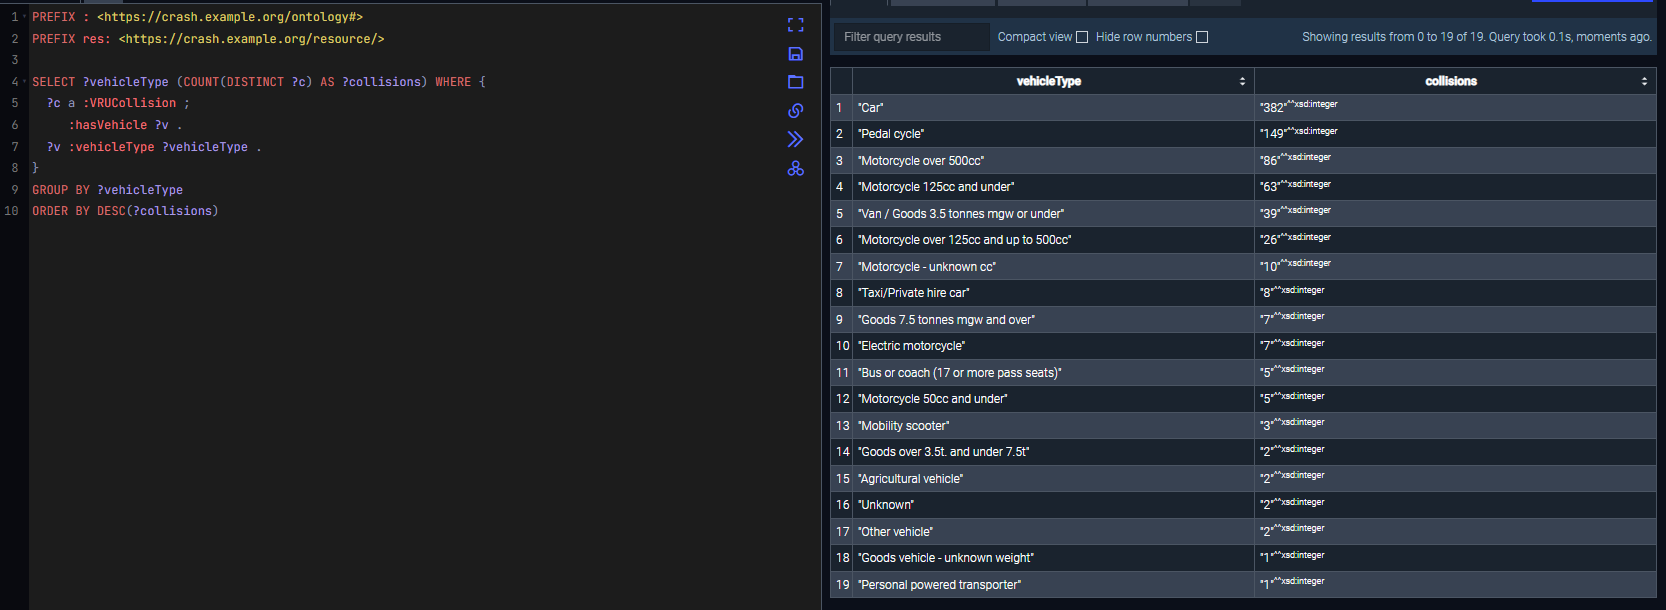
\includegraphics[width=\linewidth]{q2.png}\caption{Q2 in GraphDB.}\end{figure}
\textbf{Observed:} 19 rows, same as expected: Car 382, Pedal cycle 149, Motorcycle over 500cc 86, Motorcycle 125cc and under 63.

\subsection*{Q3. Top five local authorities for serious or fatal collisions on A roads in wet or icy conditions (CQ2).}
\textbf{Features:} FILTER, aggregation, multi-hop, inference (KSICollision).
\begin{lstlisting}
SELECT ?localAuthority (COUNT(DISTINCT ?c) AS ?ksi) WHERE {
  ?c a :KSICollision ; :roadClass "A" ; :surfaceCondition ?s ; :occurredIn ?l .
  FILTER(?s IN ("Wet or damp", "Frost or ice"))
  ?l :partOf ?la . ?la a :LocalAuthority ; :areaName ?localAuthority .
} GROUP BY ?localAuthority ORDER BY DESC(?ksi) LIMIT 5
\end{lstlisting}
\begin{figure}[H]\centering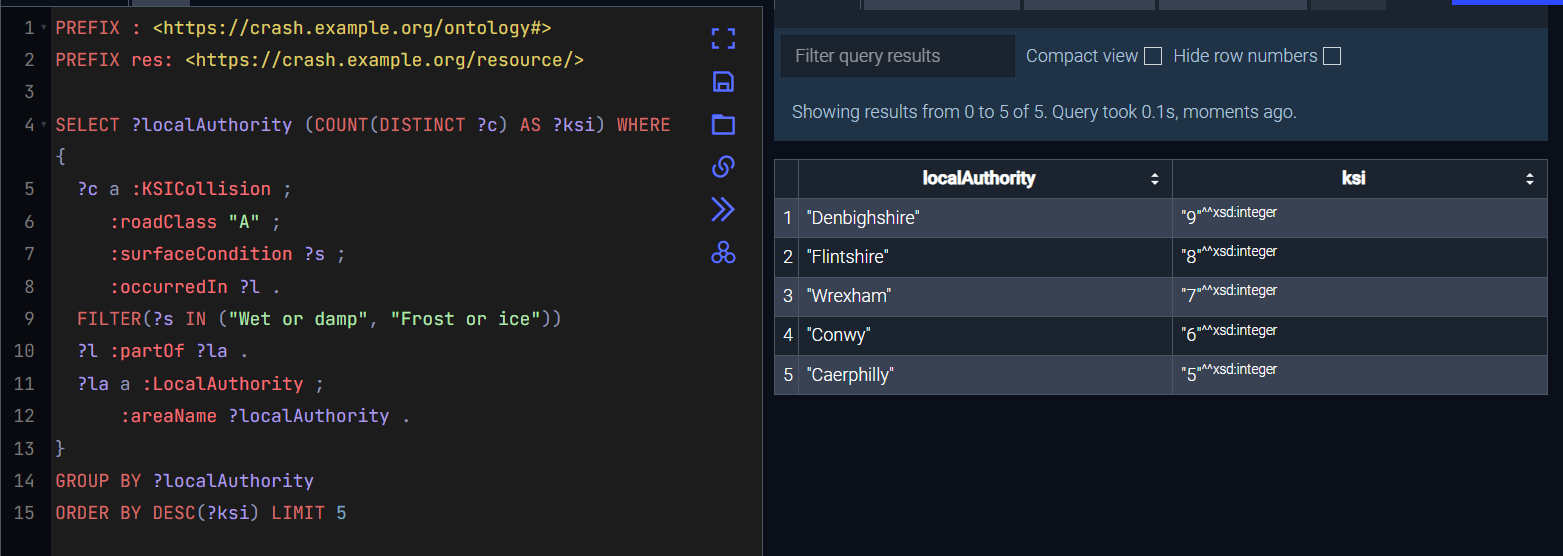
\includegraphics[width=\linewidth]{q3.png}\caption{Q3 in GraphDB.}\end{figure}
\textbf{Observed:} 5 rows, same as expected: Denbighshire 9, Flintshire 8, Wrexham 7, Conwy 6, Caerphilly 5.

\subsection*{Q4. High-risk LSOAs with their local authority and police force (CQ3).}
\textbf{Features:} property path (partOf+), multi-hop, aggregation, inference (R7, transitive partOf).
\begin{lstlisting}
SELECT ?lsoa ?localAuthority ?force (COUNT(DISTINCT ?c) AS ?ksi) WHERE {
  ?l a :HighRiskArea ; :areaCode ?lsoa ; :partOf+ ?pf .
  ?pf a :PoliceForce ; :areaName ?force .
  ?l :partOf ?la . ?la a :LocalAuthority ; :areaName ?localAuthority .
  ?c a :KSICollision ; :occurredIn ?l .
} GROUP BY ?lsoa ?localAuthority ?force ORDER BY DESC(?ksi) ?lsoa
\end{lstlisting}
\begin{figure}[H]\centering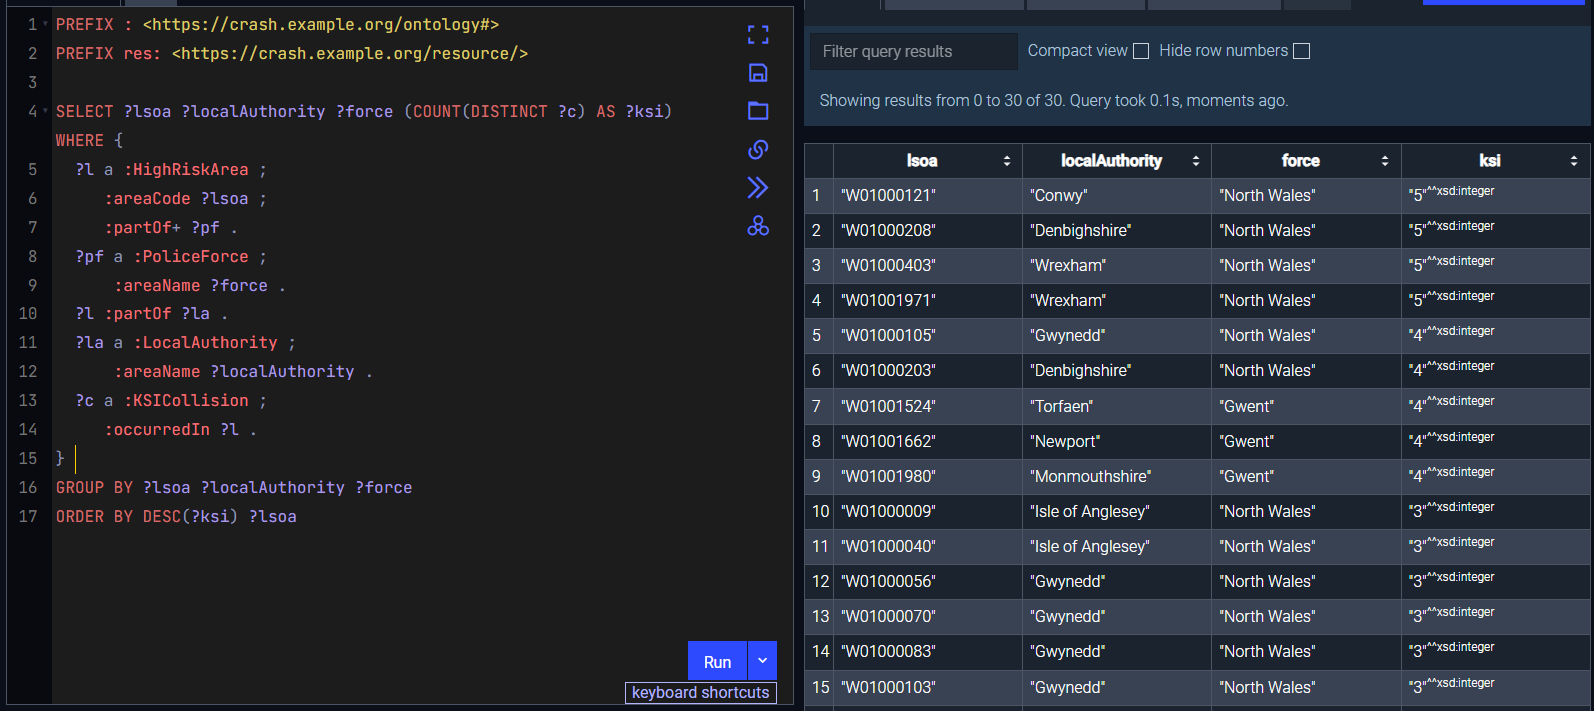
\includegraphics[width=\linewidth]{q4.png}\caption{Q4 in GraphDB.}\end{figure}
\textbf{Observed:} 30 rows, same as expected. Top: W01000121 Conwy 5, W01000208 Denbighshire 5, W01000403 Wrexham 5, W01001971 Wrexham 5. Gwent LSOAs appear too (W01001524 Torfaen 4).

\subsection*{Q5. Fatal or serious pedestrian and cyclist casualties.}
\textbf{Features:} UNION, FILTER, aggregation, inference (subclasses).
\begin{lstlisting}
SELECT ?type (COUNT(DISTINCT ?x) AS ?casualties) WHERE {
  { ?x a :Pedestrian . BIND("Pedestrian" AS ?type) }
  UNION
  { ?x a :Cyclist . BIND("Cyclist" AS ?type) }
  ?x :casualtySeverity ?sev .
  FILTER(?sev IN ("Fatal", "Serious"))
} GROUP BY ?type
\end{lstlisting}
\begin{figure}[H]\centering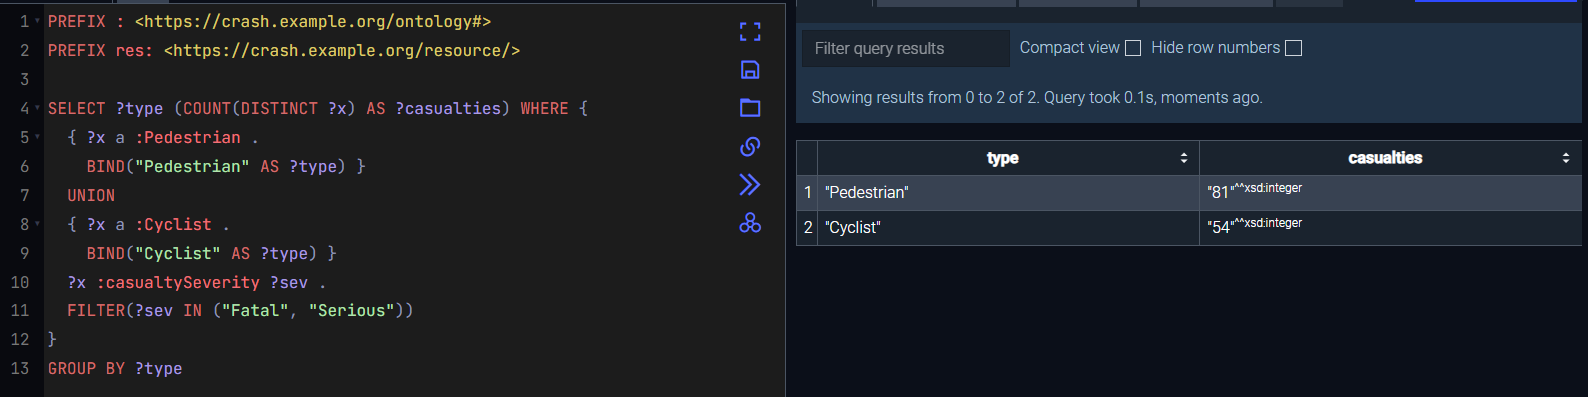
\includegraphics[width=\linewidth]{q5.png}\caption{Q5 in GraphDB.}\end{figure}
\textbf{Observed:} 2 rows, same as expected: Pedestrian 81, Cyclist 54.

\subsection*{Q6. High-risk LSOAs per local authority, keeping authorities with none.}
\textbf{Features:} OPTIONAL, aggregation, inference (R7).
\begin{lstlisting}
SELECT ?localAuthority (COUNT(DISTINCT ?l) AS ?highRiskLSOAs) WHERE {
  ?la a :LocalAuthority ; :areaName ?localAuthority .
  OPTIONAL { ?l :partOf ?la ; a :HighRiskArea . }
} GROUP BY ?localAuthority ORDER BY DESC(?highRiskLSOAs) ?localAuthority
\end{lstlisting}
\begin{figure}[H]\centering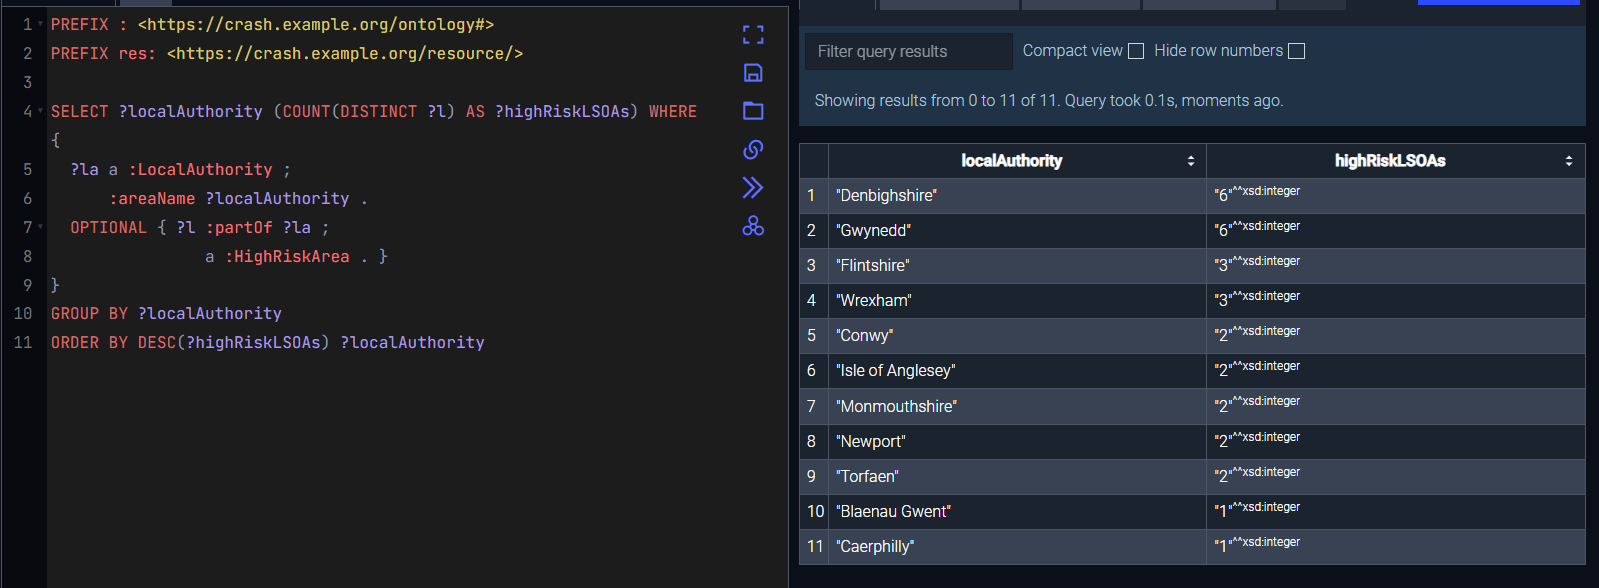
\includegraphics[width=\linewidth]{q6.png}\caption{Q6 in GraphDB.}\end{figure}
\textbf{Observed:} 11 rows, same as expected (sum 30): Denbighshire 6, Gwynedd 6, Flintshire 3, Wrexham 3. No authority has 0, so OPTIONAL drops no rows here.

\subsection*{Q7. Gwent serious or fatal collisions and how many involved a vulnerable road user (CQ6).}
\textbf{Features:} property path (occurredIn/partOf+), OPTIONAL, aggregation, inference.
\begin{lstlisting}
SELECT (COUNT(DISTINCT ?c) AS ?ksi) (COUNT(DISTINCT ?vru) AS ?withVRU) WHERE {
  ?c a :KSICollision ; :occurredIn/:partOf+ ?pf .
  ?pf a :PoliceForce ; :areaName "Gwent" .
  OPTIONAL { ?c a :VRUCollision . BIND(?c AS ?vru) }
}
\end{lstlisting}
\begin{figure}[H]\centering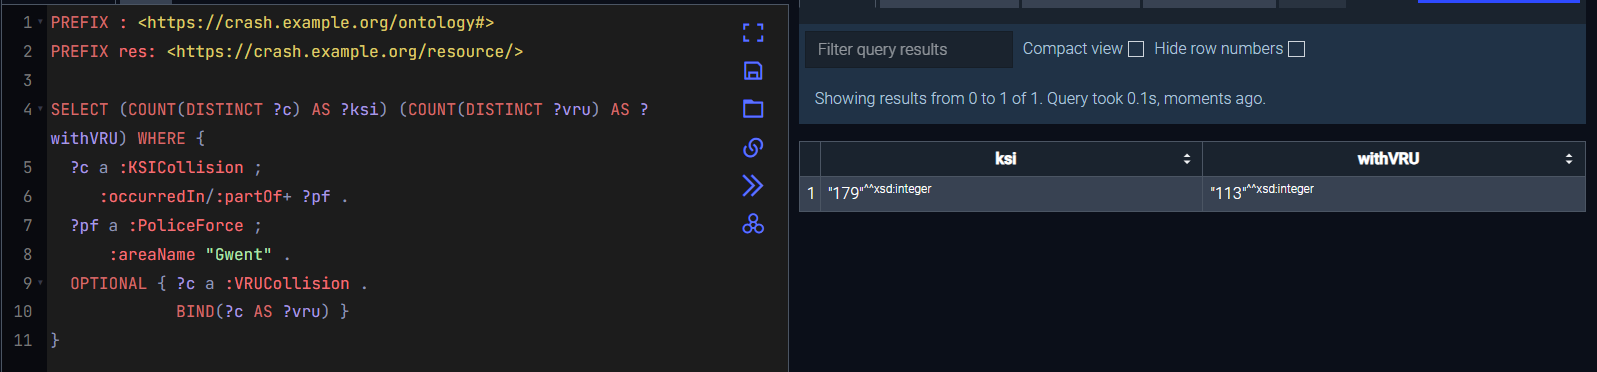
\includegraphics[width=\linewidth]{q7.png}\caption{Q7 in GraphDB.}\end{figure}
\textbf{Observed:} 1 row, same as expected: 179 KSI collisions, 113 with a vulnerable road user.

\subsection*{Q8. Serious or fatal collisions with a vulnerable road user in each high-risk LSOA (CQ13).}
\textbf{Features:} multi-hop, aggregation, inference (three derived classes).
\begin{lstlisting}
SELECT ?lsoa (COUNT(DISTINCT ?c) AS ?ksiVRU) WHERE {
  ?l a :HighRiskArea ; :areaCode ?lsoa .
  ?c a :KSICollision , :VRUCollision ; :occurredIn ?l .
} GROUP BY ?lsoa ORDER BY DESC(?ksiVRU) ?lsoa
\end{lstlisting}
\begin{figure}[H]\centering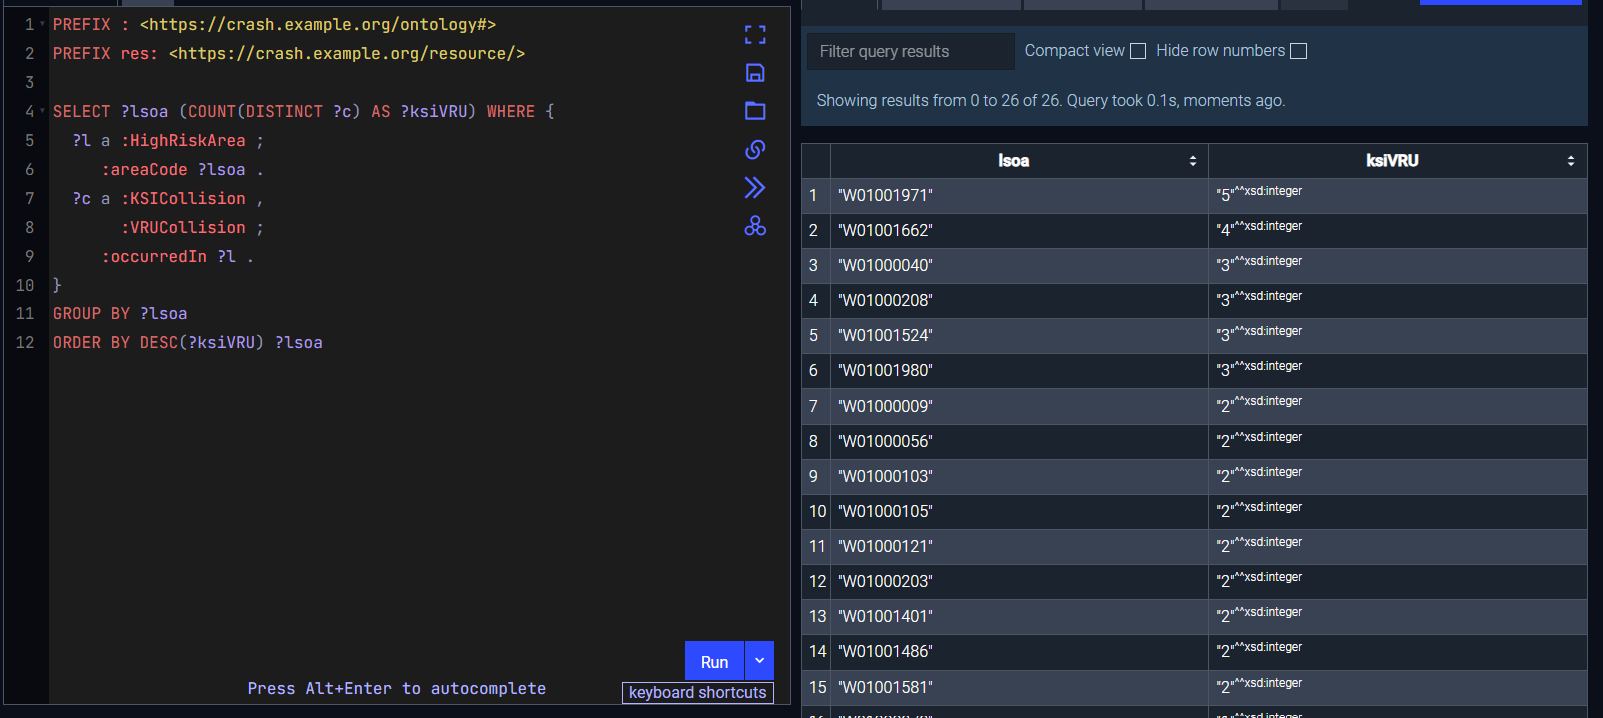
\includegraphics[width=\linewidth]{q8.png}\caption{Q8 in GraphDB.}\end{figure}
\textbf{Observed:} 26 rows, same as expected. Top: W01001971 5, W01001662 4, then four LSOAs with 3.

\subsection*{Q9. Full record of one collision: vehicle, casualty, local authority and police force (CQ12).}
\textbf{Features:} multi-hop (3 hops), property path, basic pattern.
\begin{lstlisting}
SELECT ?c ?light ?weather ?vehicleType ?casualty ?severity ?la ?force WHERE {
  BIND(res:Collision_202560C002220 AS ?c)
  ?c :lightCondition ?light ; :weatherCondition ?weather ; :hasVehicle ?v ;
     :occurredIn/:partOf ?laIri .
  ?v :vehicleType ?vehicleType .
  ?v :hasCasualty ?x . ?x :casualtySeverity ?severity .
  ?laIri :areaName ?la ; :partOf ?pf . ?pf :areaName ?force .
  BIND(STRAFTER(STR(?x), "resource/") AS ?casualty)
}
\end{lstlisting}
\begin{figure}[H]\centering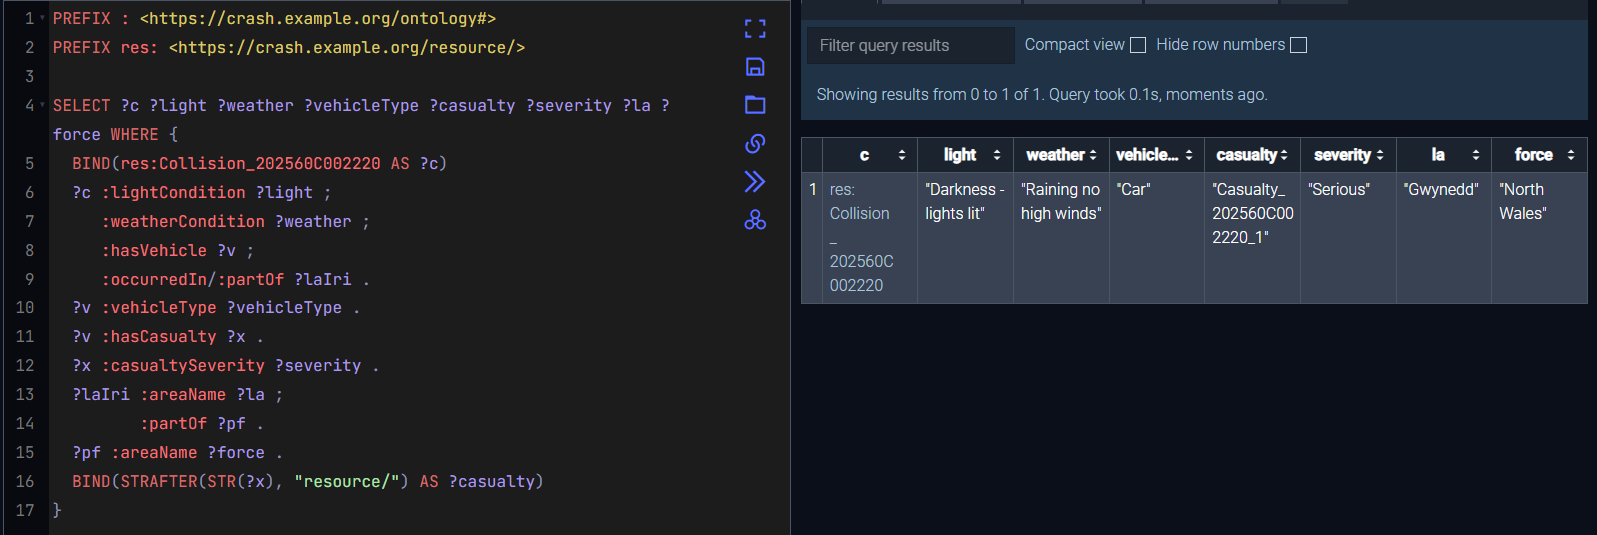
\includegraphics[width=\linewidth]{q9.png}\caption{Q9 in GraphDB.}\end{figure}
\textbf{Observed:} 1 row, same as expected: Darkness - lights lit, Raining no high winds, Car, Casualty\_202560C002220\_1, Serious, Gwynedd, North Wales.

\subsection*{Q10. Motorcyclists seriously or fatally injured on roads with a limit of 50 or more (CQ10).}
\textbf{Features:} FILTER, multi-hop via inferred involvesCasualty, inference.
\begin{lstlisting}
SELECT ?c ?speed ?severity WHERE {
  ?c a :KSICollision ; :speedLimit ?speed ; :involvesCasualty ?x .
  ?x a :Motorcyclist ; :casualtySeverity ?severity .
  FILTER(?speed >= 50 && ?severity IN ("Fatal","Serious"))
} ORDER BY DESC(?speed) ?c
\end{lstlisting}
\begin{figure}[H]\centering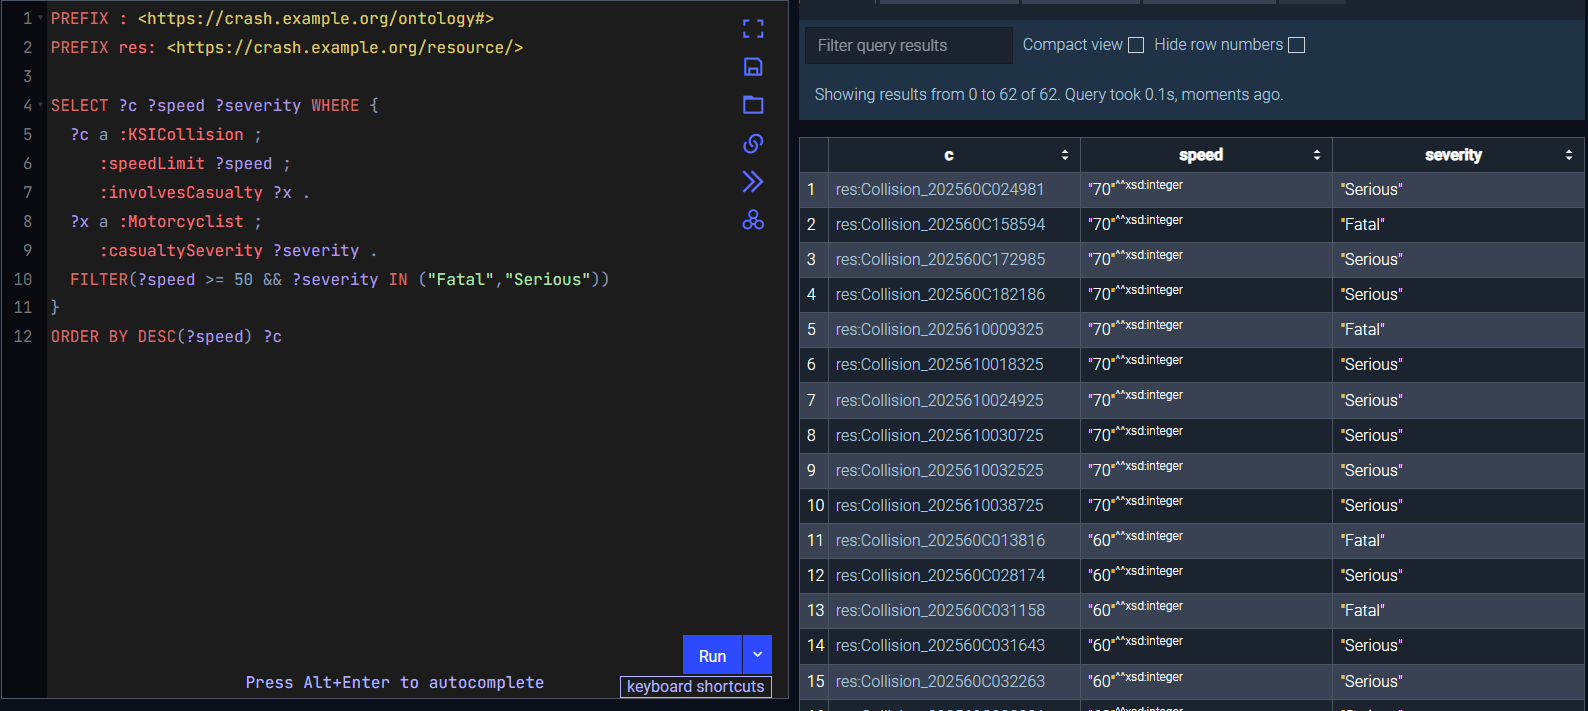
\includegraphics[width=\linewidth]{q10.png}\caption{Q10 in GraphDB.}\end{figure}
\textbf{Observed:} 62 rows, same as expected. First row Collision\_202560C024981 (70, Serious), second Collision\_202560C158594 (70, Fatal).

\section{Inference examples}
Each example shows the explicit facts stored in \texttt{crash\_data.ttl}, the schema rule, and the fact that the reasoner adds. None of the inferred facts is in the data file.
\subsection*{Example 1: SeriousCollision becomes KSICollision (R1)}
\begin{tabular}{L{3cm} L{12.5cm}}
\toprule
Explicit fact & \texttt{res:Collision\_202560C000676 a :SeriousCollision}\\
Rule / schema & \texttt{:KSICollision owl:equivalentClass [ owl:unionOf (:FatalCollision :SeriousCollision) ]}; \texttt{:SeriousCollision rdfs:subClassOf :Collision}\\
Inferred fact & \texttt{res:Collision\_202560C000676 a :KSICollision}\\
\bottomrule\end{tabular}
\begin{lstlisting}
SELECT ?type WHERE { res:Collision_202560C000676 a ?type .
  FILTER(STRSTARTS(STR(?type), "https://crash.example.org/ontology#")) }
\end{lstlisting}
\begin{figure}[H]\centering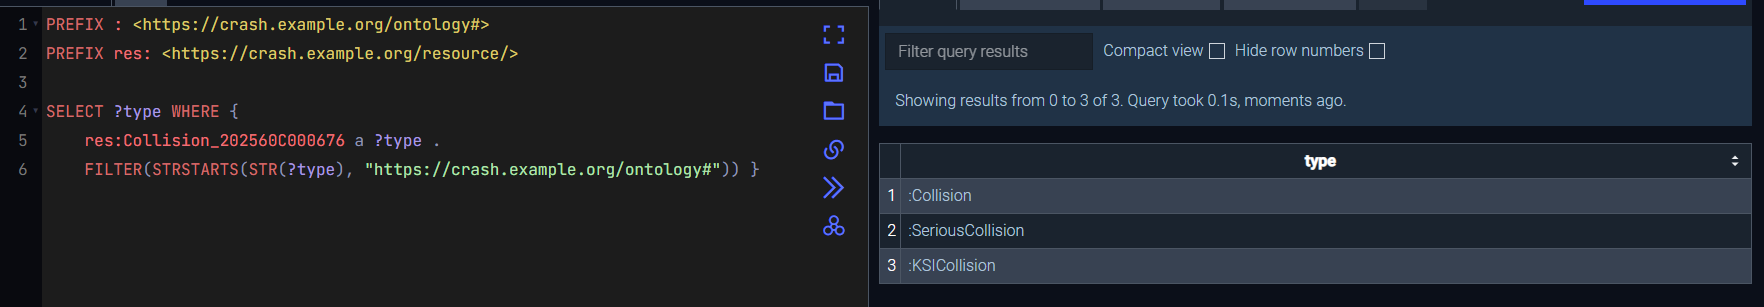
\includegraphics[width=\linewidth]{inf1.png}\caption{Observed: Collision, SeriousCollision and the inferred KSICollision.}\end{figure}
\subsection*{Example 2: pedestrian casualty makes the collision a VRUCollision (R3, R4, R6)}
\begin{tabular}{L{3cm} L{12.5cm}}
\toprule
Explicit facts & \texttt{res:Collision\_2025610052425 :hasVehicle res:Vehicle\_2025610052425\_1}; \texttt{res:Vehicle\_2025610052425\_1 :hasCasualty res:Casualty\_2025610052425\_1}; \texttt{res:Casualty\_2025610052425\_1 a :Pedestrian}; the collision is \texttt{a :SeriousCollision}\\
Rule / schema & \texttt{:Pedestrian rdfs:subClassOf :VulnerableRoadUser}; \texttt{:involvesCasualty owl:propertyChainAxiom (:hasVehicle :hasCasualty)}; \texttt{:VRUCollision} $\equiv$ \texttt{:involvesCasualty some :VulnerableRoadUser}\\
Inferred facts & \texttt{Casualty\_2025610052425\_1 a :VulnerableRoadUser}; \texttt{Collision\_2025610052425 :involvesCasualty Casualty\_2025610052425\_1}; \texttt{Collision\_2025610052425 a :VRUCollision} and \texttt{a :KSICollision}\\
\bottomrule\end{tabular}
\begin{lstlisting}
SELECT ?c ?x WHERE {
  VALUES ?c { res:Collision_2025610052425 }
  ?c a :VRUCollision , :KSICollision ; :involvesCasualty ?x .
  ?x a :VulnerableRoadUser .
}
\end{lstlisting}
\begin{figure}[H]\centering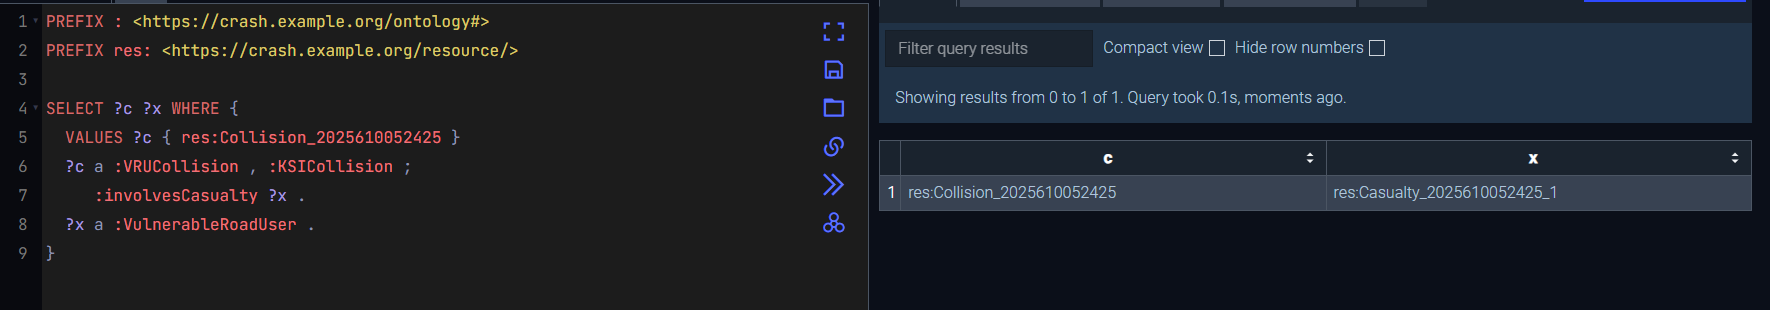
\includegraphics[width=\linewidth]{inf2.png}\caption{Observed: one row, the collision and its casualty.}\end{figure}
\subsection*{Example 3: partOf chain to the police force (R5) and HighRiskArea (R7)}
\begin{tabular}{L{3cm} L{12.5cm}}
\toprule
Explicit facts & \texttt{res:LSOA\_W01001662 :partOf res:LA\_W06000022}; \texttt{res:LA\_W06000022 :partOf res:PoliceForce\_61} (Gwent); at least four KSI collisions occurred in this LSOA (Q4 shows 4)\\
Rule / schema & \texttt{:partOf a owl:TransitiveProperty} (R5); R7 INSERT: an LSOA with at least 3 KSI collisions gets \texttt{a :HighRiskArea}\\
Inferred facts & \texttt{res:LSOA\_W01001662 :partOf res:PoliceForce\_61}; \texttt{res:LSOA\_W01001662 a :HighRiskArea}\\
\bottomrule\end{tabular}
\begin{lstlisting}
SELECT ?l ?pf WHERE { res:LSOA_W01001662 a :HighRiskArea ; :partOf ?pf . ?pf a :PoliceForce }
\end{lstlisting}
\begin{figure}[H]\centering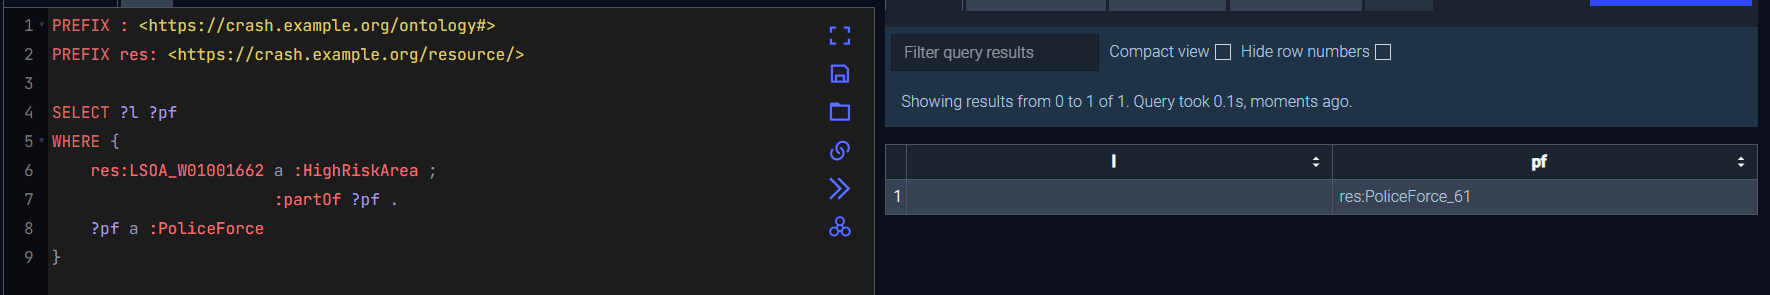
\includegraphics[width=\linewidth]{inf3.png}\caption{Observed: one row with PoliceForce\_61. The \texttt{?l} column is empty only because the LSOA IRI is written into the pattern instead of bound to \texttt{?l}; \texttt{SELECT ?pf} would be cleaner.}\end{figure}
\end{document}